\documentclass[conference]{IEEEtran}
%\documentclass[journal]{IEEEtran}
\usepackage{graphicx}
%\documentclass[]{article}

%\usepackage{draftwatermark}\SetWatermarkText{Not For Distribution}
%\SetWatermarkScale{2}\SetWatermarkLightness{0.85}

\newcommand{\ppv}{P_{pv}}
\newcommand{\pinv}{P_{inv}}

\title{Title}

\begin{document}

%\abstract{}

%\author{
%\IEEEauthorblockN{Daniel Soto}
%\IEEEauthorblockA{
%The Earth Institute\\
%Columbia University\\
%New York, NY 10027}
%\and
%\IEEEauthorblockN{Vijay Modi}
%\IEEEauthorblockA{
%Department of Mechanical Engineering\\
%Columbia, University\\
%New York, NY  10027}
%}

\maketitle

\begin{abstract}
Conventional solar generation architectures using photovoltaic
panels, sealed lead acid batteries, and inverters show room for
cost improvement.
Using data collected from photovoltaic microgrid users and simulations
we demonstrate potential cost reductions using alternate 
technologies and architectures.
\end{abstract}

\section{Introduction}

The cost of renewable and distributed energy systems must be
optimized to sustainably provide electricity to the customers 
beyond the reach of the grid.
Private energy service companies (ESCOs) may be able to supply power
where utilities have failed to reach.
However, as private companies, ESCOs will be especially sensitive
to the price of generation and the ability to collect
tariffs.
This constraint makes it necessary to optimize energy systems
for cost.
Since these systems are often paid for by the revenue collected
from electricity sales, these optimizations are important.
\cite{fee for service literature}
Our previous work has focused on the improved collection of 
tariffs through mobile commerce and prepayment \cite{ICTD}.
This work will focus on potential cost reductions which allow
the same level of energy to be delivered for a lower total
investment and cost per kWh.

Our observations of electricity use in newly electrified villages
show usage patterns that are difficult to serve efficiently 
with existing technology.
Our data show that villages whose primary electricity use is 
lighting, television, and cell phone charging have wide variation
in power.
This work presents opportunities for efficiency and therefore
cost reduction in the areas of power conversion and storage.
These recommendations are based on data collected from customers
who have recently been provided with a near-grid-quality
electrical connection and are paying for that power on a
per kilowatt-hour basis.
There are many optimizations of system size in the literature
\cite{optimizations}.
This work adds to the literature by considering the effects
of the time of day of usage and the efficiencies of commonly
used inverters and batteries.
Conventional inverters cannot service this variation in power
at a consistent efficiency.
This decrease in efficiency leads to an increase in both
generation and storage costs.

Two approaches to mitigation of this load variation exist, 
the first is scheduling or addition of loads that smooth consumption.
The second approach is developing a power converter architecture
that is less sensitive to the variation in loads.
We present data addressing the first approach, where two of our 
sites have added freezers.
Our microgrid data and simulations show that these daytime loads
can increase the cost-effectiveness of a microgrid.
We show the load duration curve with the addition of these 
devices and the effect on overall efficiency.
For the second approach we model the cost reductions possible
for a hypothetical inverter that has a more constant efficiency
across all loads in its operating range.
This could be achieved through multiple inverters with 
different operating regimes or future improvements in inverter
technology.
Modest gains are available through load management or 
inverter efficiency.
The biggest gains are possible as battery technologies improve.

We model the system cost using existing sealed lead acid 
battery technology and promising Lithium and Lead Carbon
technologies.
The improved efficiency and lifetimes of these emerging technologies
can significantly reduce the cost of off-grid electricity
where per kWh costs are currently dominated by the need
for storage.


\section{Microgrid and Data Description}
The simulations in this paper will use data collected from 
Mali.
This section describes the microgrid systems that this data
is taken from.
It will also describe some of the notable features in the data.

\subsection{Data collection}
We have installed 17 microgrid systems with remote connectivity
in Mali and Uganda \cite{ICTD}.
Each of these systems consists of a 1.4 kWp array of photovoltaic
panels with a 48 V, 360 Ah battery bank.
An MPPT charge controller handles battery charging and a
750 W inverter supplies the microgrid with 50 Hz, 220 V power.
Up to 20 customers are connected to these systems in a star
topology where each customer has a dedicated wire to the
central facility.
Each customer is metered by a commercially available device that
allows for energy measurement and reporting and a switch to
automatically connect or disconnect the consumer.
These systems send data on an hourly basis to a central server
using SMS messages.
Data is collected on the energy consumption of each household
as well as the AC energy consumption of the entire system.
From the solar controller, we measure and store hourly information
on the solar energy delivered to the system and the battery
voltage.

\subsection{Timeseries Description}
These messages allow us to create a database of timeseries
information from the customers.
For most customers, the peak power is consumed in the evening
as shown in Figure \ref{two-bulb-profile}.
Most of the customers have little or no usage during the day time.
The system however, uses about 50W to run the metering, computation,
and communication electronics giving a similar profile but with
a larger daytime use.

\begin{figure}[h]
\begin{center}
% 93bc6d og ghtc2012.py
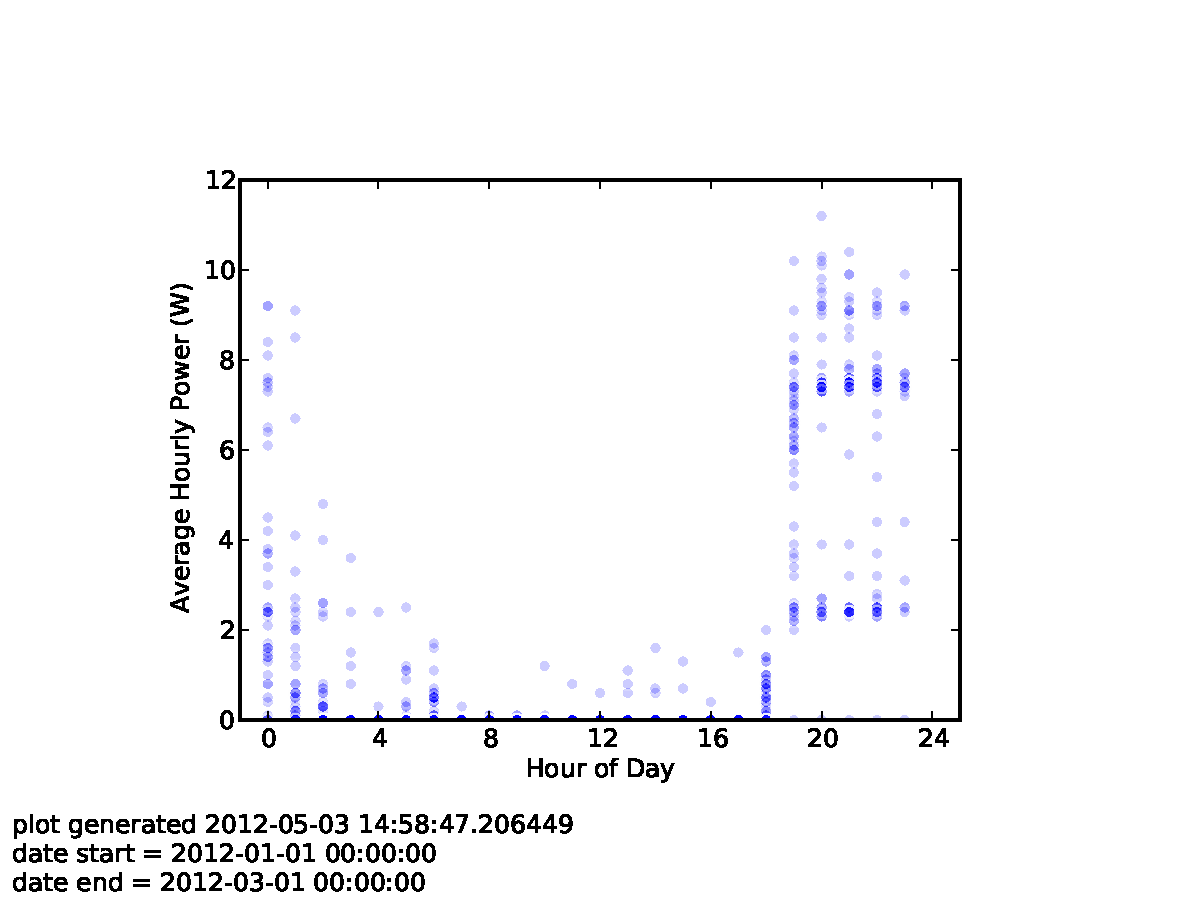
\includegraphics[trim = 0.7in 0.8in 0.7in 1.1in, clip, width=\columnwidth]
{figures/two_bulb_profile.pdf}
\end{center}
\caption{Customer exhibiting two bulb lighting load.
Each data point is the hourly load for a single day.
Multiple days are superimposed.
Points are transparent so that frequent measurements appear darker.
This customer displays two common evening power levels corresponding
to the use of one or two lightbulbs.
This not that this customer has very small power use during the day.}
\label{two-bulb-profile}
\end{figure}

We have provided two freezers that customers are using to
sell ice or frozen drinks.
The hourly profile for the household using this freezer
is shown in Figure \ref{freezer}.
These freezers draw a much larger amount of power than the
typical lighting load and have a lower variation when measured
on an hourly basis.

\begin{figure}[]
\begin{center}
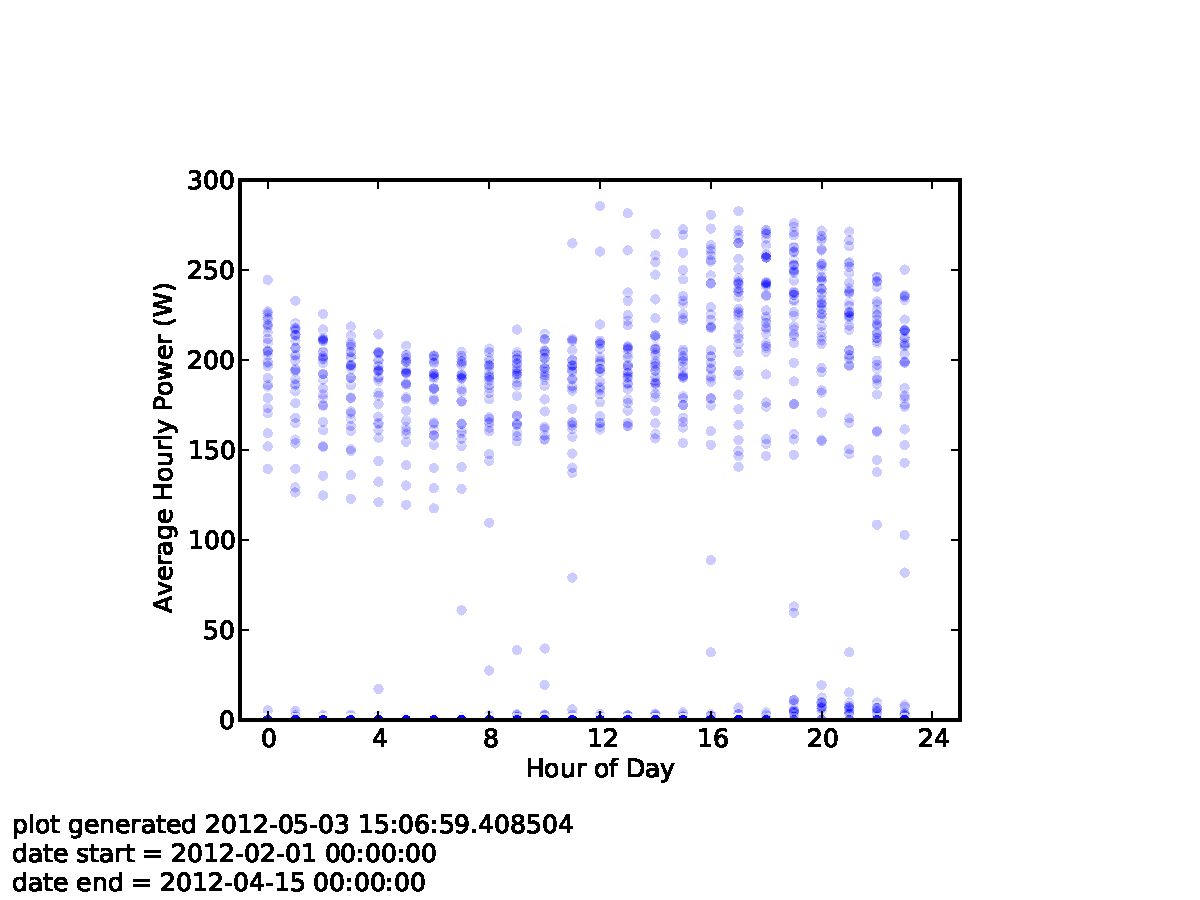
\includegraphics[trim = 0.7in 0.8in 0.7in 1.1in, clip, width=\columnwidth]{figures/freezer_profile.pdf}
\end{center}
\caption{Circuit with freezer.  
Power use is much more consistent.}
\label{freezer}
\end{figure}

\subsection{Load Duration Curves}
If we sort the hourly power demand over a long time period, we
construct a curve called a load duration curve \cite{REEPS}.
A load-duration curve (Figure \ref{two_ldc}) shows this variation.
In the microgrid (ml07) that does not have a freezer, the most common
power level is less than 50W, which is well below the peak
efficiency of the inverter.
For the system that does have a freezer, the system spends the bulk
of its time consuming on the order of 200W, which is much closer
to the peak efficiency operating point of the inverter.
The inverter is sized so that the maximum customer load is safely
accommodated by the inverter.
However, there is a substantial efficiency penalty for operating the
inverter below the optimal point.

We can express these loads in terms of the capacity factor,
where the capacity factor is relative to the rated output
of the inverter.
Systems with high power variability will lose efficiency since
the system will often be operated outside of the range of
peak efficiency.

\begin{figure}[h]
\begin{center}
% og ghtc2012.py 07d761 plot_two_ldc()
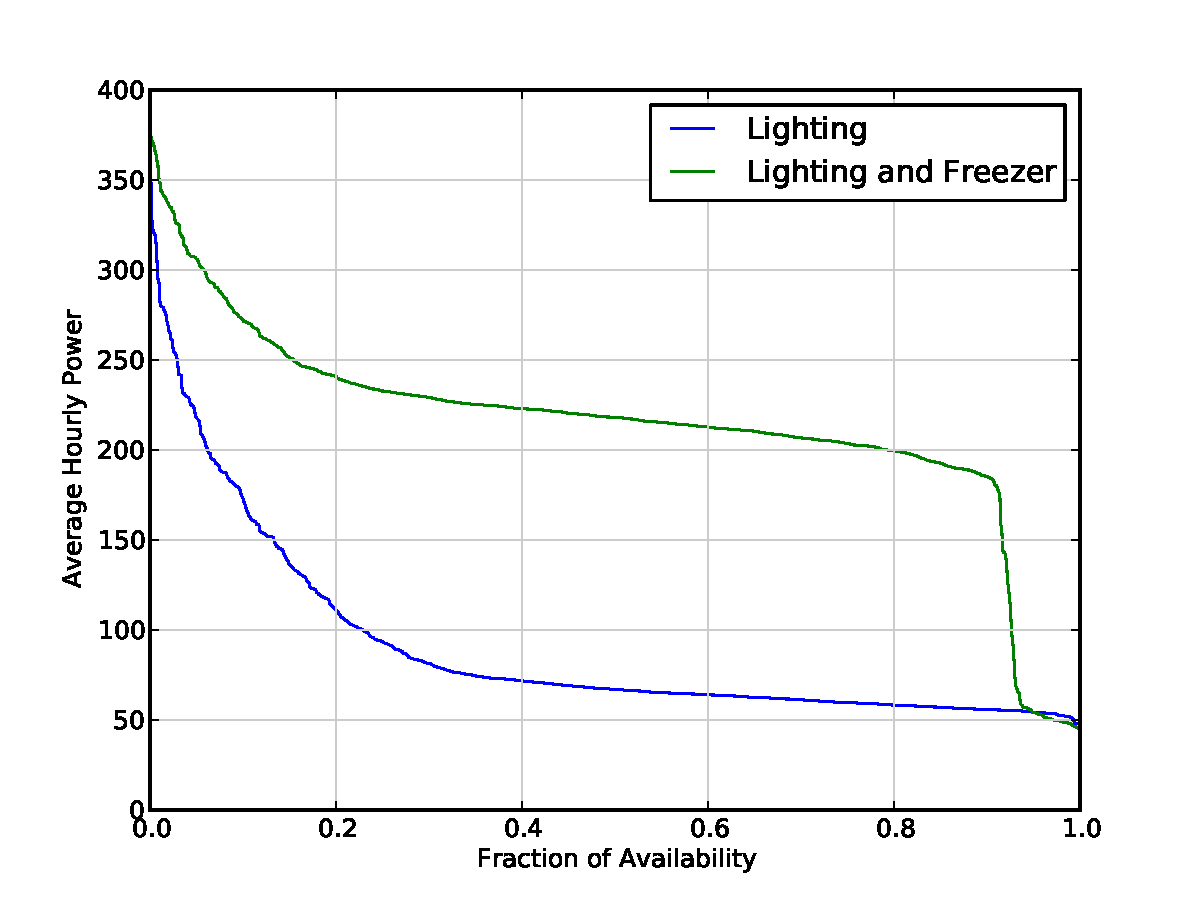
\includegraphics[trim = 0.0in 0.2in 0.0in 0.5in, clip, width=\columnwidth]{figures/two_ldc.pdf}
\end{center}
\caption{Load duration curve for two typical microgrid systems,
including metering, computing, and computation.
Inverter and charge controller consumption is not included.
One system includes a significant daytime refrigeration load,
while the other does not.
}
\label{two_ldc}
\end{figure}

\subsection{Overall System Efficiency}

We can estimate an overall system efficiency from the
usage data and information from the solar controller
on photovoltaic energy generation.
This estimate of the overall efficiency of the system
is defined as power delivered by solar
power controller divided by the power delivered to the system.
We do not include the parasitic power consumed by the electronics.

Our data shows that as the capacity factor of the inverter
increases, the overall system efficiency improves.

The large variations in loads exhibited by these customers prompted
us to investigate the impact on system efficiency that these
loads are causing.
We pursued both a measurement of the systems and a simulation approach.

\begin{table}
\centering
\begin{tabular}{c c c}
Meter & System Utilization Factor & System Efficiency \\
\hline
ml03 & 0.38 & 0.62 \\
ml05 & 0.33 & 0.69 \\
ml06 (freezer) & 0.54 & 0.88 \\
ml08 (freezer) & 0.55 & 0.90 \\
\end{tabular}
\caption{System Utilization and system efficiency}
\label{efficiency}
\end{table}

In ML06, which has considerable daily load, we see an overall
efficiency of 0.89.
In ML05, with much less daily load, the overall efficiency
is 0.78.

\section{Simulation Description}

We examine the effect of load variation and alternate technologies
on the size and cost of the system by creating an 
energy simulation of the system.
The simulation finds the minimum panel size and battery capacity
that will meet the demand assuming clear-sky radiation.
This model is intended to allow comparisons between systems and
load profiles rather than provide accurate guidance for system
sizes over a typical meteorological year.
The simulation takes as input the hourly load profile from a
set of either real or hypothetical customers.
The model then uses a series of assumptions on battery and solar
panel parameters to calculate the power and storage at each hour.
The battery is considered to be a simple energy storage device
with perfect efficiency during charging and an efficiency of
$\eta_B$ on discharge.
We can calculate the energy in the battery in discrete time
steps according to the following equation.
%
$$ E_B(t+\Delta t) = E_B(t)
                   + P_{charge} \cdot \Delta t
                   - \frac{P_{discharge} \cdot \Delta t}{\eta_B}
                   $$
%
Where $P_{charge}$ is the power flow when the photovoltaic
production is greater than the inverter demand and
$P_{discharge}$ is the power flow when the inverter demand
is greater than the photovoltaic power available.
They are given by the following equations.
%
$$ P_{charge} = \left\{
			  \begin{array}{rl}
			  0 & \pinv > \ppv \\
			  \ppv - \pinv & \pinv < \ppv
			  \end{array}
			  \right. $$
%
$$ P_{discharge} = \left\{
			  \begin{array}{rl}
			  \pinv - \ppv & \pinv > \ppv \\
			  0 & \pinv < \ppv
			  \end{array}
			  \right. $$
%
The power demanded by the inverter is calculated using the efficiency
of the inverter as a function of temperature according to
$$ \pinv = \frac{P_{AC}}{\eta_{inv}(P_{AC})} $$
%
Where $P_{AC}$ is the hourly power demanded by the consumers of the microgrid.

The difference equation is run in a loop where the 
panel size in the model is adjusted until the energy remaining
in the battery at the end of the simulation is equal to the
energy at the start of the simulation.
The minimum battery size is then the peak-to-peak variation
of the battery energy time series.
A time series trace is shown in Figure \ref{simulation}.
Once the simulation finds a solution where the starting and final
storage are equal, the model outputs the minimum battery size
to meet the storage need at 100\% depth of discharge and the 
minimum solar panel size to meet the demand.
Based on panel size and battery size output along with the 
assumptions on panel cost and battery cost and life, the model 
predicts the net present value (NPV) of the system over the 
life of the system.
In this model we use a 7\% discount factor and a 20-year time
horizon.
The battery assumptions for these simulations are listed in 
Table \ref{table_battery_assumptions} and the panel assumptions 
are listed in Table \ref{table_panel_assumptions}.

\begin{figure}[h]
\begin{center}
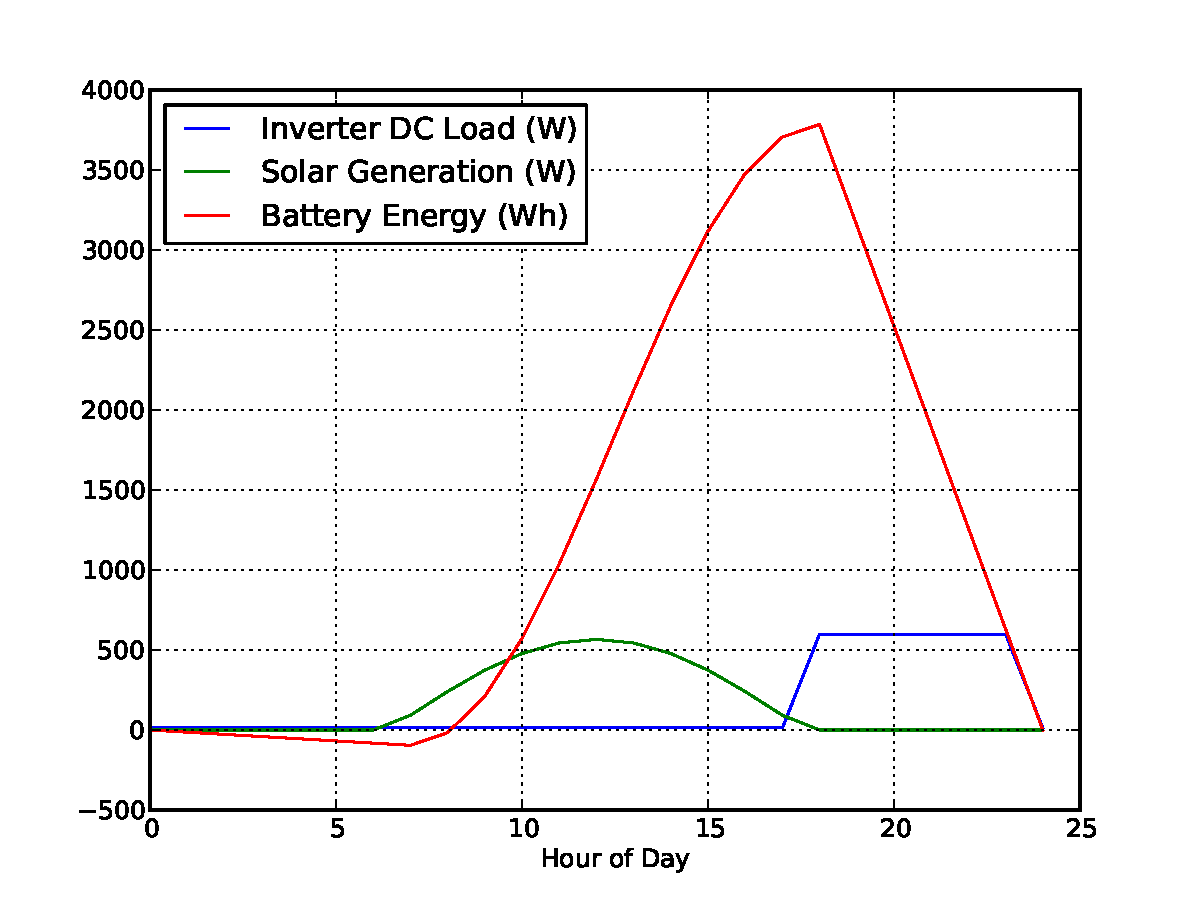
\includegraphics[trim = 0.0in 0.2in 0.0in 0.5in, clip, width=\columnwidth]{figures/simulation.pdf}
\end{center}
\caption{
Time series of simulation.
}
\label{simulation}
\end{figure}

\begin{table*}
\centering
\begin{tabular}{ c c c c c }
Battery Chemistry & Initial Cost & Lifetime & Optimal & Storage \\ 
                  & (USD/kWh)    & (yr)     & DOD     & Efficiency\\
Sealed Lead Acid (SLA)       & \$140  & 2  &  50\%  & 75\%  \\
Lithium Iron Phosphate (LFP) & \$1000 & 6  & 100\%  & 95\%  \\ 
Lead Carbon (PbC)            & \$140  & 6  &  50\%  & 75\%  \\
\end{tabular}
\caption{Battery Assumptions for Modeling.}
\label{table_battery_assumptions}
\end{table*}

\begin{table}
\centering
\begin{tabular}{ c c }
Panel Efficiency       & 13.5\% \\
Panel Latitude         & 14 N  \\ 
Panel Cost             & \$1/W  \\
Panel Lifetime         & 20 years \\
\end{tabular}
\caption{Solar Panel Assumptions for Modeling.}
\label{table_panel_assumptions}
\end{table}


\section{Calculation Results and Discussion}

The simulation results compare the performance of hypothetical
systems to the baseline system and report potential improvements.

\subsection{Baseline System}
The simulated baseline system is based on the system we have
installed in the field.
The inverter efficiency for this baseline system is shown in Figure
\ref{inverter_curves} as the ``Baseline'' curve.
The battery used in the baseline system is the Sealed Lead Acid
battery in Table \ref{table_battery_assumptions}.
The solar panel assumptions used in the baseline and all other
simulations are listed in Tabel \ref{table_panel_assumptions}.
This baseline system is used for comparison against the
improvements discussed below.

\begin{figure}[]
\begin{center}
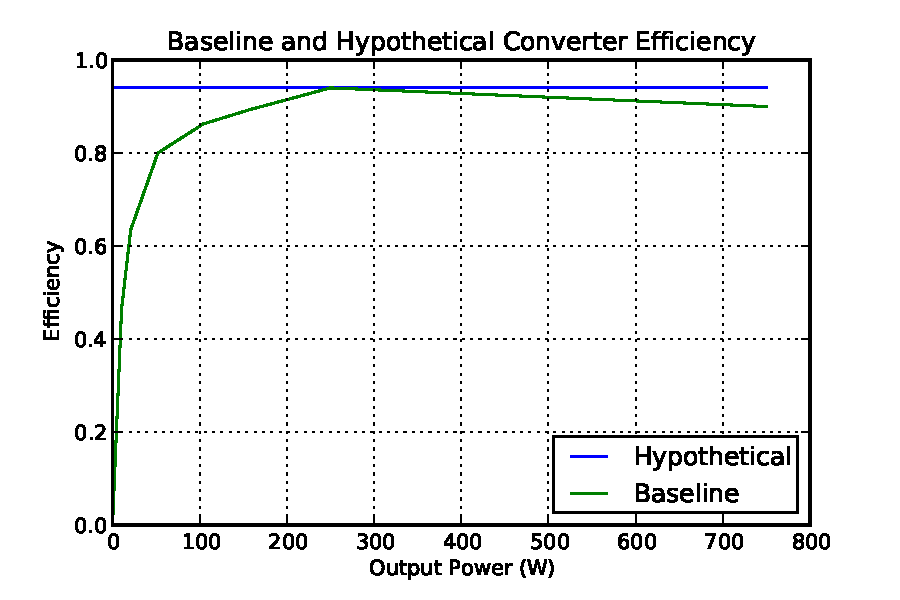
\includegraphics[width=\columnwidth]{figures/inverter_curves.pdf}
\end{center}
\caption{Efficiency curves for baseline and proposed system.}
\label{inverter_curves}
\end{figure}

\subsection{Impact of time of load on system size}

The storage and generation necessary to service a given daily
amount of energy can vary depending on what time of day
that energy is delivered.
To demonstrate the effect of the time of day that power
is consumed on the generation and storage capacity of the system,
we calculate the panel and battery size for four loads with
the same total daily energy but occurring at different times of day.
We define a nighttime load that has the entire day's load 
occurring between 6pm and midnight.
We also define a daytime load that occurs between 9am and 3pm 
and a constant load that is evenly spread across the entire day.

In addition to these three hypothetical loads, we also use loads
representative of the measured customer loads at our microgrids. 
The ``Lighting'' village load uses a representative day from one of the
village microgrids and has a small constant load and a large
nighttime load.
The ``Freezer'' village load is from one of our microgrids using a freezer
to provide ice for sale.

%Table \ref{tbl_baseline} 
Figure \ref{fig_baseline} 
shows the results of simulations
which demonstrate the variability of panel size and battery
size with the type of load.
The lowest total cost is delivered for the ``Day'' load
since there is very little storage necessary.
The highest total cost is incurred for the ``Night'' load since
the storage demand is the greatest.
There are variations in the size and price of the panel
necessary to meet the load, but the cost impact is small
compared to the storage costs.


\begin{figure}[]
\begin{center}
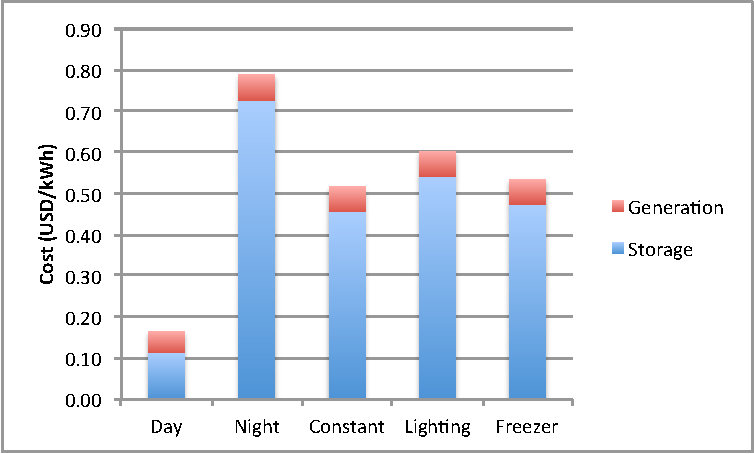
\includegraphics[width=\columnwidth]{figures/baseline.pdf}
\end{center}
\caption{Cost of electricity for different load profiles using Baseline 
inverter and battery system and hypothetical and measured loads.}
\label{fig_baseline}
\end{figure}

\begin{table*}
\centering
\begin{tabular}{c c c c c}
Configuration & Panel Capacity & Minimum Battery & Battery NPV & Solar NPV \\
              & (kWp)          & Size (kWh)      & (USD)       & (USD)     \\
\hline
% village_simulation 845102 table_2()
typical day lead acid          & 0.59 & 0.76 & 1306 & 595 \\
typical night lead acid        & 0.74 & 4.92 & 8421 & 738 \\
typical continuous lead acid   & 0.70 & 3.08 & 5281 & 704 \\
typical village lead acid      & 0.73 & 3.66 & 6270 & 727 \\
\end{tabular}
\caption{Impact of load time-of-day on system size.
Loads are normalized to 3.0 kWh per day.}
\label{tbl_baseline}
\end{table*}

\subsection{Inverter Efficiency}

A typical inverter is inefficient at loads below its
preferred operating point.
If the load is usually close to this high efficiency
point, the lower efficiencies at low power are not important.
If however, as we observe, there is a high variability
in the power output where daytime loads are very small
but evening loads are greater, this inefficiency can have
a significant impact.

If the system is run inefficiently during the daytime, the inefficiency
burden only impacts the amount of generation capacity needed.
If the system is run inefficiently during the evening, both the
generation and the storage costs are affected, multiplying the
penalty.
Late-night and early morning cellphone charging and vampire
loads can cause this inefficiency.

To demonstrate this effect, we run our simulation with
a hypothetical power conversion device that has an
efficiency equal to the peak efficiency of the baseline
inverter at any power level.

%Table \ref{table_inverter} 
Figure \ref{fig_inverter}
shows the in delivered price for loads that
are often below peak, such as the measured village load
and the continuous load.

\begin{figure}[]
\begin{center}
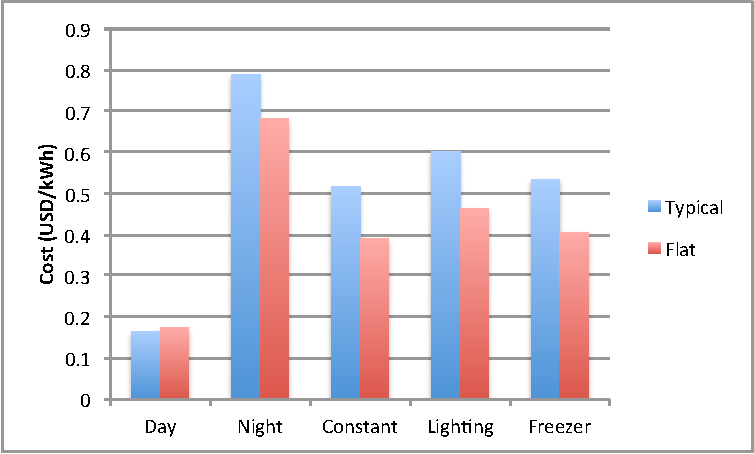
\includegraphics[width=\columnwidth]{figures/inverter.pdf}
\end{center}
\caption{Cost of electricity for different load profiles using Baseline 
inverter and battery system and hypothetical and measured loads.}
\label{fig_inverter}
\end{figure}


\begin{table*}
\centering
\begin{tabular}{c c c c c}
Configuration & Panel Capacity & Minimum Battery & Battery NPV & Solar NPV \\
              & (kWp)          & Size (kWh)      & (USD)       & (USD)     \\
\hline
% village simulation f19442 table_3
flat day lead acid             & 0.50 & 0.88 & 1509 & 498 \\
flat night lead acid           & 0.62 & 4.26 & 7289 & 621 \\
flat continuous lead acid      & 0.53 & 2.33 & 3993 & 532 \\
flat village lead acid         & 0.55 & 2.81 & 4819 & 553 \\
\end{tabular}
\caption{Impact of inverter non-ideality on system size}
\label{table_inverter}
\end{table*}

\subsection{Battery Chemistry}

The initial battery cost is given by

$$ C_B = E_{storage} \frac{1}{\eta_B} \frac{1}{DOD_{optimal}} c_B $$

Where $E_{storage}$ is the storage necessary, $\eta_B$ is the
round trip energy efficiency, $DOD_{optimal}$ is the desired
operating point of the battery for long life, and $c_B$ is the
initial cost of the battery per kWh.
A very important metric however is the life cycle cost of the 
battery replacement which depends on the cycle life of the battery.

New battery chemistries could reduce the fraction of investment
that goes toward storage of electricity.
The incumbent battery technology is sealed lead acid.
Emerging technologies of interest are Lithium Iron Phosphate
and Lead Carbon.

Relative to sealed lead acid batteries, LiFePO batteries 
have better cycle life, higher specific cost, and better
turnaround efficiency.
PbC batteries are not yet mature but have improved cycle
life and likely similar specific cost and turnaround
efficiency.
The assumptions for the battery types in the simulation
are found in Table \ref{table_battery_assumptions}.
We simulate the impact of these on system size and total cost
in Table \ref{table_battery}.
For the case of typical village data, the lifetime cost of 
lead acid and LFP are similar.
If PbC batteries are able to maintain their cost while
improving cycle life, they will provide a clear improvement
in the life-cycle cost.


\begin{table*}[!t]
\centering
\begin{tabular}{ c c c c c }
Configuration & Panel Capacity & Minimum Battery & Battery NPV & Solar NPV \\
              & (kWp)          & Size (kWh)      & (USD)       & (USD)     \\
\hline
%table 5
% village simulation c4e80b table_5()
typical village lead acid      & 0.73 & 3.66 & 6270 & 727 \\
typical village LFP            & 0.62 & 2.93 & 7043 & 615 \\
typical village lead carbon    & 0.73 & 3.66 & 2466 & 727 \\
\end{tabular}
\caption{Simulation results for battery chemistries.
Net present value is calculated at 7\% over 20 year 
time horizon.}
\label{table_battery}
\end{table*}


\section{Discussion / Future Work}
While the simulation results discussed are speculative, 
we believe that experimentation in this regime is important.




\section{Summary}
Hourly demand data for newly electificed communities has been gathered.
We find that improving no-load and low load power consumption of the
inverter can reduce storage and generation needs.

Since the storage costs are greater than generation and BOS costs
for off-grid solar, the largest cost reductions could come from
Lead Carbon batteries.
If LFP improvements continue, they could become competitive in the
future.



technology \& cost improvement from baseline \\
slaved inverters    \& xx\% \\
LFP battery         \& xx\% \\
Lead Carbon Battery \& xx\% \\


\begin{thebibliography}{1}
\bibitem{optimizations}
Z Wissem, K Gueorgui, K H\'edi,
Modeling and techinical--economic optimization of an autonomous
photovoltaic system,
Energy, Vol. 37, 2012 pp. 263-272
(doi:10.1016/j.energy.2011.11.036)
\bibitem{ICTD}
D.~Soto, SharedSolar. ICTD 2012.
\bibitem{REEPS}
G.~Masters,
"Renewable and Efficient Electric Power Systems",
Wiley Interscience,
2004
\end{thebibliography}


\end{document}

%---------------------------------------------------------------------------%
%---------------------------------------------------------------------------%
%---------------------------------------------------------------------------%
%---------------------------------------------------------------------------%
%---------------------------------------------------------------------------%
%---------------------------------------------------------------------------%
%---------------------------------------------------------------------------%
%---------------------------------------------------------------------------%
%---------------------------------------------------------------------------%
%---------------------------------------------------------------------------%
%---------------------------------------------------------------------------%
%---------------------------------------------------------------------------%



We have measured the load patterns of users and have generated
load-duration curves over a N-day period.
From this curve, (Figure \ref{ldc}) we estimate the overall
efficiency of the inverter.
$$ \sum p_i / \eta_i $$
The overall inverter efficiency is much lower than its rated
efficiency because the inverter is operated for so much time
at a low fraction of its capacity.


%$$ \ppv = insolation \cdot array size \cdot array efficiency
%         \cdot controller efficiency $$


We can simulate the effective inverter efficiency for a given
load profile and inverter curve.

$$ \eta_{effective} = \frac{\sum P_{AC} \cdot \Delta t}
                          {\sum P_{AC} /\eta_{inv} \cdot \Delta t} $$

While lithium batteries are a factor of XX more expensive
than lead-acid batteries based on the capacity of the battery
(USD/kWh), the cost per delivered watt-hour of electricity
over the lifetime of the battery is comparable.
Additional economic improvement is gained by lower weight
for shipping and improved round trip efficiency which lowers
both the battery capacity and the generation capacity when nighttime
loads are needed.


\subsection{DC Distribution}

Since both the generation and consumption of electricity in our
sites is in the form of DC electricity, it is natural to
question the necessity of the inverter.
In addition to inefficiency of conversion from DC to AC at the
generation side and from AC to DC at the consumption side,
these DC loads have less than unity power factor which further
lowers the efficiency of the inverter.
In areas where connection to the grid is extremely unlikely
in the future, an all DC distribution system is worthy of
serious consideration.

If the efficiency curve of a DC/DC converter were favorable,
a high-voltage direct current (HVDC) distribution scheme could
be used.
Our testing of a 48 VDC to 12 VDC converter is over 80\% for
the range of power of interest.
The no-load dissipation for this device was below our measurement
capacity of 0.5W.

\subsection{Mitigating Load Variation}
Systems with better no-load performance should be used to counteract
the problem of efficiency at the lower end.

Two solutions exist for this problem, the first is to remove
the constant loads (meter electronics, communication, and
computing) from the inverter.
This could allow an inverter to operate in a power-down or
search mode for most of the time and then switch on only
to service loads.

\subsection{Slaved inverters}
A chain of inverters that turn on in a cascaded fashion could
be more efficient.

\subsection{Inverters with Standby Mode}
The standby loss could be low but an small use will energize the
entire system.




\subsection{Distributed Storage}
Another possibility is local storage at the home with a small inverter
that the customer only switches on during times when power
is needed.
This reduces the standby load to zero but likely adds to the
fixed cost of the system.